\documentclass[12pt]{article}
\usepackage[utf8]{inputenc}
\usepackage{amsmath}
\usepackage{graphicx}
\usepackage{float}
\graphicspath{  {./Figures/}  } 
\setcounter{secnumdepth}{4}
\setcounter{tocdepth}{4}

% ========== Title Page ==========
\title{Thin Walled Pressure Vessel}
\author{
	\textbf{Submitted by}: \\
	Henry V. Gilbert \\
	The University of Tennessee Knoxville \\
	hgilber1@vols.utk.edu \\
	(931) - 335 - 0669 \\
	960 Riverside Forest Way
	Apt. 002 \\
	Knoxville TN, 37915\\ \\ \\ \\ \\ \\ \\ 
	\textbf{Submitted to: }\\ 
	Dr. Seyedreza Djeddi \\
	Research Assistant Professor and Lecturer \\
	Tickle College of Engineering, MABE Department \\
	314 Perkins Hall \\
	1506 Middle Drive \\
	Knoxville TN, 37996 \\
	}
\date {Feburary 19 2019}
\begin{document}
\maketitle

\newpage
\section*{Letter of Transmittal}
Dr. Seyedreza Djeddi \\
Research Assistant Professor and Lecturer \\
Tickle College of Engineering, MABE Department \\
314 Perkins Hall \\
1506 Middle Drive \\
Knoxville TN, 37996 \\ \\
Dear Dr. Djeddi: \\ 

In this packet I am submitting a formal lab report for the thin walled pressure vessel experiment, 
conducted under your supervision. This experiment studied the relationship between stress and
strain using a thin walled pressure vessel. Based on theoretical equations, the hoop and 
axial stress can be determined knowing the pressure vessel radius, wall thickness, and internal
pressure. Experimentally, one can determine the internal stresses using strain transformations,
principal strains, and Hooke's law. The acquired strain data allowed us to determine that Rosettes A 
and B were the least accurate, and Rosettes C and D were highly accurate in measuring 
principal stresses. The data analysis involved comparing measured normalized strain relationships,
measured principal stresses to theoretical principal stresses, and measured hoop stress to 
measured axial stress. Most of the data followed a linear trend, so the inconsistencies in Rosettes A 
and B were precise but not accurate. \\  \\ \\ \\  \\ \\ \\ \\ 
\\ 
Sincerely, \\
Henry V. Gilbert. \\ \\ 
Enclosed: Thin-walled pressure vessel report. 

% ========== Executive Summary ==========
\section*{Executive Summary}
The goal of this laboratory experiment was to understand the process of measuring stress. Unfortunately, stress gages do not exist. To counter this lack of direct measurement, 
experimentally measuring stress is accomplished through the stress-strain relationship found in Hooke's law. Hooke's law states that stress is related to strain through the material properties E, Young's Modulus of Elasticity, and $\nu$, Poisson's ratio.

Using a thin walled pressure vessel, this procedure enabled not only the measurement of stress, but also the ability to check the accuracy of these measurements. Based on the thin wall pressure vessel theory, axial and hoop stresses can be calculated using the thin-walled cylinder approximation. These equations,  $\sigma_{hoop} = \frac{pr}{t} $  and  $\sigma_{long} = \frac{pr}{2t} $ , relate applied internal  pressure to principal stresses. Based on this, the strains (and therefore stresses) experienced from direct control of internal pressure can be validated from the cylinder pressure vessel theory. 

% Summary of data interpretations
For the stress measurements, a unitless resemblance ratio, R*, was approximated by $\frac{measured}{theoretical} $. Here, a 1.00 resemblance would mean perfectly identical data, while anything higher than 1.0 would show that measured data was higher than theoretical, and lower than 1.0 means measured was lower than theoretical.
The calculations showed that rosettes C and D were the most accurate. Rosette C had an average of R*=0.93  to theoretical axial stress, and Rosette D had an average R* = 1.06  to theoretical axial stress and an average R*=1.03 to theoretical hoop stress.  Rosette A had an average R*= 0.69 axial, and R*=0.75 hoop. Rosette B had a R*=0.59 and R*= 0.73 similarity to theoretical axial and hoop stress, respectively. The experiment validated the cylinder stress thin-wall approximation, as well as the strain-to-stress data reduction process. 

% Limitations and conclusions 
Recall that the cylindrical stress equations are only theoretical. In this case, the data received
from rosette D most closely represented the true stresses. The theoretical cylindrical stresses rely on the assumption that internal pressures are perfectly uniformly distributed. Also one must consider
the age of the equipment and the effect of fatigue on the pressure vessel. With the hand pump, the
pressure 50 psig, 100 psig, etc. represented the \textit{internal} pressure. In a thin walled vessel, the maximum stress will occur at the inside of the wall, and decrease to its minimum on the outside of the wall. This means that our strain rosettes were measuring only the \textit{lowest} value of the stress state.


\newpage
\tableofcontents
% LO symbols
% List of Figures
% LO Tables
\newpage

\newpage
\listoffigures
\section{List of Figures}

\newpage
\listoftables
\section{List of Tables}


\newpage
\section*{List of Symbols}
\begin{figure}[H]
	\centering
	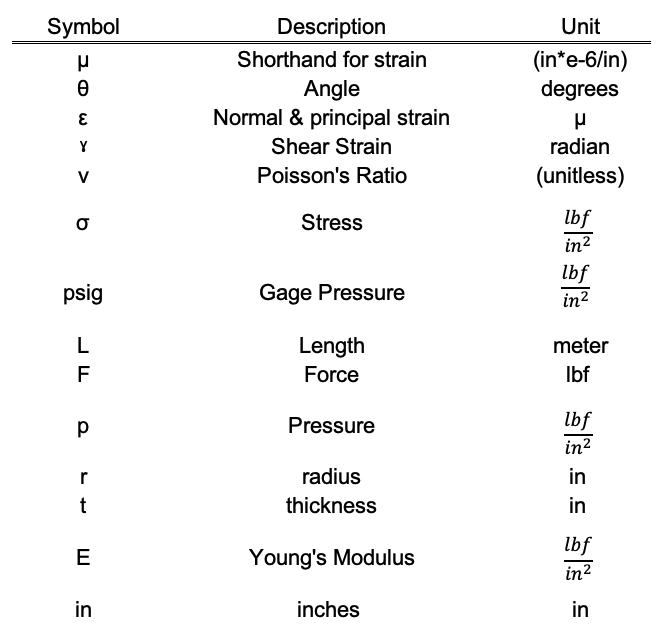
\includegraphics[width=0.9\textwidth]{symbols}
\end{figure}
\newpage




\section{Introduction}
\paragraph{Background} 
Pressure vessels find themselves in modern engineering applications across various fields. These 
engineering feats help astronauts, and supply scuba divers with the precious breath of life during
underwater missions. Anyone who loves cooking with propane and propane accessories understands the 
vital need of a pressured container for the precious gas. With pressure vessels, trapping the ever-expanding
gaseous molecules is a thing of ease. 

Strain, $\epsilon$, is a measure of deformity in an object. It is defined as 
$$ \epsilon = \frac {\Delta L}{L_0}$$
The value of the resultant strain applied to an object is a function of its material properties, mainly
Young's Modulus of Elasticity, E. This property defines a materials elasticity, and is the ratio of the 
applied stress to its deformation, given in the equation $ \frac{F}{\epsilon} = E  $. However, these equations
are only relevant during tensile testing. In two and three dimensional states of applied stress, a more 
complex derivation occurs to give the equations :  \\
This experiment explores the effect of applied pressure to a thin walled pressure vessel. A pressure 
vessel is defined as "thin" if the ratio of its total diameter to wall thickness is greater than 20. Here, assuming that the 
internal stresses are constant and uniform,   [1].

\paragraph{Objectives}
The primary objective in this experiment was to relate the theoretical stress calculations in a cylindrical
pressure vessel from the equation $\sigma_{hoop} = \frac{pr}{t} $  and  $\sigma_{long} = \frac{pr}{2t} $, to the
process of obtaining stresses from strain measurements. 
Once the measured strain values were converted to principal stresses, data analysis was used to 
check the validity of the data. Among these calculations was comparing the measured stresses to 
the theoretical values. 

% ========== Methodology ==========
\newpage
\section{Methodology}
\paragraph{General Overview} 
With the pressure vessel apparatus, strain rosettes were attached to various locations along the vessel. 
Once the strain values were measured, principal stresses were calculated using Hooke's law. The 
principal stresses obtained from Hooke's law were graphed and compared to theoretical
values. Checks were put in place to determine the validity of the strain gage readings. Note: All configuration 
figures are derived from reference [2]. 

\paragraph {Apparatus}

\begin{figure} [H]
	\centering
	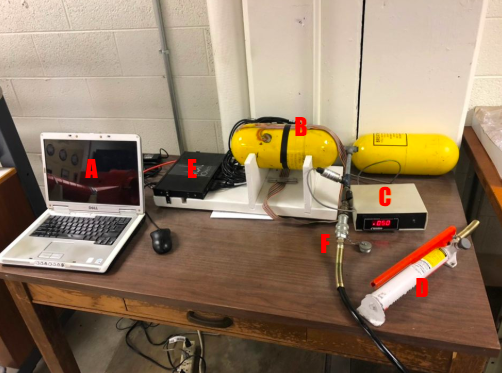
\includegraphics[width=0.9\textwidth]{setup}
	\caption{\textbf{Overhead view of the experiment configuration}}
\end{figure}
Figure 1 shows the full setup for the pressure vessel experiment, with red letters "A-F" to 
label individual components. Letter A represents the Dell Latitude data acquisition machine. The
Excel program was used here to store the measured data. "B" is the MIT-C-5435 oxygen tank, with 
strain rosettes configured on it as shown in \textbf{Figure 2}. "C" is the OMEGA DP-350 pressure
indicator, which retrieves data from "E", the IOtech-6224 strain gage input module, attached to
"F", the OMEGA PX302-500GV pressure transducer. Label D corresponds to the hydraulic hand pump 
that was manually used to control the oxygen tank's internal pressure. 

% Black and white picture of the rosette configurations. Reference to the lab handouts. 
\begin{figure} [H]
	\centering
	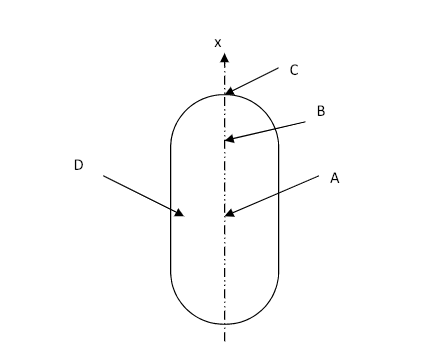
\includegraphics [width=0.4\textwidth]{vessel}
	\caption{\textbf{Overview of the pressure vessel rosette configuration}}
\end{figure} 

% Strain rosette angle configurations. 
\begin{figure} [H]
	\centering
	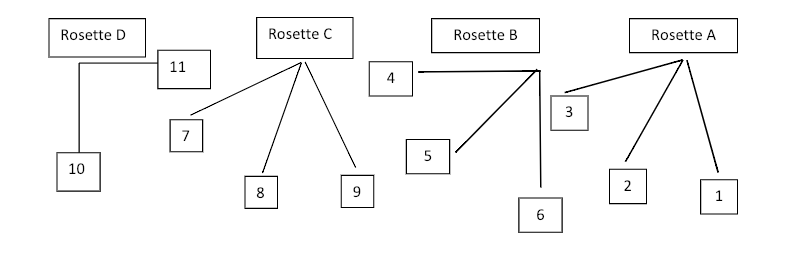
\includegraphics [width=0.9\textwidth]{rosettes}
	\caption{ \textbf{Strain Rosette Configurations}}
\end{figure} 
Shown in \textbf{Figure 3} is the configuration of each strain rosette, and \textbf{Figure 4} shows
the angle values which belong to each strain gage. These angles are measured counterclockwise from the 
x axis. 

Based on the configuration above, the gage pairs (4 \& 11) and (6 \& 10)  will detect the same strain value. Therefore, 
\begin{align}
\epsilon_{4} = \epsilon_{11} \\
\epsilon_{6} = \epsilon_{10} 
\end{align}
\\ \\ Rosette D's average value of strain should be equal to the strain read on gage 5, shown in 
\begin{align}
2\times\epsilon_{5} = \epsilon_{10} + \epsilon_{11}
\end{align}
Due to rosette C's placement on the axial end, there will be only a one dimensional state of strain recorded. Therefore, the values detected in all gages should be equal. 
\begin{align}
\epsilon_{7} = \epsilon{_8} = \epsilon_{9} 
\end{align}

\begin{figure} [H]
	\centering
	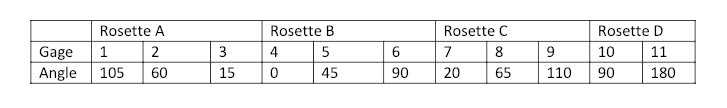
\includegraphics [width=1.0\textwidth]{gage_angles}
	\caption{ \textbf{Strain Rosette Angles}}
\end{figure} 

% Explain each rosette, angles, and possible similarities. 


\paragraph{Test Procedure}
Starting at 0 psig, a hand pump was used to increase the pressure by 50 psig increments. Once the pressure was set, a mean strain gage was shot selected in the data acquisition program, capturing an instantaneous 
state of mean strain. At 0 psig, theoretically, there should
be zero stress and strain in the vessel. However, strain gages work by measuring micro displacements, and some
minor effects of gravity, age, and physical configuration can cause the voltage at 0 psig to give a value of strain. To
compensate this linear offset, a "normalized" set of data was used, in which every set of data was subtracted from the
zero offset measurement. For example, instead of the strain reading at 100 psig being the raw values pulled from
the data acquisition system, the strain value from 100 psig would be captured, then the difference between the 
baseline value at 0 psig would be subtracted from 100 psig, and the resulting value would be the normalized value. For example, at 100 psig, $ \epsilon_{100} = \epsilon_{100 measured} - \epsilon_0 $. \textit{All calculations used the normalized strain measurements at each pressure increment.} This process
was repeated for each strain measurement up to 400 psig. After the ascending measurements were taken, the 
hand pump had its pressure released, and the strain values from 400 psig to 0 psig were taken, in 50 psig decrements, to determine the descending sets of data. 


\paragraph {Data Reduction Procedure }
The overall flow of data starts at nominal strains, transformed to plane strains, converted  to
principal strains, and finally, through Hooke's law, converted to principal stresses. Once the measured 
principal stresses were obtained, they are  classified as either hoop or axial stresses. For rosettes A, B, and D,
the hoop stress is the larger value, and the axial stress is the smaller value.The corresponding $\theta_i$ values for each gage come from \textbf{Figure 4}. 

Starting with nominal strains, the strain transformation theory is applied to three measured strains, shown in the set of equations 
\begin{align}
\epsilon_1 = \epsilon_x\cos^{2}\theta_1 + \epsilon_y\sin^{2}\theta_1 + \gamma_{xy}\cos{\theta_1}\sin{\theta_1} \\
\epsilon_2 = \epsilon_x\cos^{2}\theta_2 + \epsilon_y\sin^{2}\theta_2 + \gamma_{xy}\cos{\theta_2}\sin{\theta_2} \\
\epsilon_3 = \epsilon_x\cos^{2}\theta_3 + \epsilon_y\sin^{2}\theta_3 + \gamma_{xy}\cos{\theta_3}\sin{\theta_3} 
\end{align}

These three equations are solved using the matrix multiplication: 
\begin{align}
\begin{bmatrix}
\epsilon_x \\
\epsilon_y \\
\gamma_{xy} \\
\end{bmatrix}
= 
\begin{bmatrix}
   \cos^{2}\theta_1 & \sin^{2}\theta_1 & \cos{\theta_1}\sin{\theta_1}  \\
   \cos^{2}\theta_2 & \sin^{2}\theta_2 & \cos{\theta_2}\sin{\theta_2}  \\
   \cos^{2}\theta_3 & \sin^{2}\theta_3 & \cos{\theta_3}\sin{\theta_3}  \\
\end{bmatrix}^{-1} \times
\begin{bmatrix}
\epsilon_1 \\
\epsilon_2 \\
\epsilon_3 \\
\end{bmatrix}
\end{align}

Once the plane strain values $\epsilon_x$, $\epsilon_x$, and $\gamma_{xy}$ are solved, the principal strains
are produced by the equations :
\begin{align}
\epsilon_{p1}, \epsilon_{p2} = \frac{\epsilon_x + \epsilon_y}{2} \pm
\frac{1}{2} \sqrt{ { \frac{\epsilon_x - \epsilon_y}{2}}^2 + {\gamma_{xy}}^2 }
\end{align}


Principal strains lead directly to the principal stresses via Hooke's law. Given the material properties of the vessel,
\begin{align}
\sigma_{p1} = \frac{E}{1-\nu^2} \big[ \epsilon_{p1} + \nu\epsilon_{p2} \big] \\
\sigma_{p2} = \frac{E}{1-\nu^2} \big[ \epsilon_{p2} + \nu\epsilon_{p1} \big]
\end{align}

Material properties for the oxygen tank were as follows: 
$$ thickness = t = 0.04 in $$
$$ radius = r =2.773 in $$
$$ Young's Modulus = E = 30 \times 10^6 psi $$ 
$$ Poisson's Ratio: \nu = 0.29 $$ 
	
\paragraph {Data Validity Checking} 
To offer a validity check to the strain gages, ratios were compared once the normalized data
was taken. From the rosette configurations, if the data were perfect, the values 
of equations (1), (2), (3), and (4) would hold perfectly true, i.e., equal 1. \\

\paragraph {Theoretical Measurements} 
Based on the thin walled pressure vessel theory, the cylinder stresses are calculated by 
\begin{align}
\sigma_{Hoop} = \frac{p\times r}{t} \\ 
\sigma_{Axial} = \frac{p\times r}{2t}
\end{align}
Thin walled pressure vessel theory only holds true if$ \frac{D}{t} > 20, $ For the vessel in this experiment, $\frac{D}{t}=\frac{5.545 in}{0.04 in} = 138$ , thus, the assumption holds true. 

\paragraph{Data Analysis}
After all the measurements were taken, three analysis methods were conducted, all involving "resemblance ratios" R*$  = \frac{\sigma_{measured}}{\sigma_{theory}} $. Here, a value of 1.0 would signify the measured data is exactly the theoretical data. Any number higher than 1.0 states that the measured value was higher than the theoretical value, and any number lower than 1.0 states that the measured value was lower than the theoretical value. For rosettes A, B, and D, where both axial and hoop stresses are present, a separate ratio was created as R* $ = \frac{\sigma_{Hoop}}{\sigma_{Axial}} $. A value of 2.0 is expected, since by definition, hoop stress is twice the value of axial stress. The three stress measurements that were analyzed were \textit{axial vs hoop}, \textit{hoop vs theoretical hoop}, and  
\textit{axial vs theoretical axial}. 
\newpage

% ================================================
% ==================== Results =====================
% ================================================
\section{Results and Discussion}\label{conclusions}
\paragraph {Results} 
Below are tables and figures representing the reduced and analyzed data from the strain rosettes and the calculated hoop and axial stresses. An important consideration is that the word "accurate" refers to closeness to the theoretical calculation, which served as the main reference state for strain measurement accuracy. 

% Strain data 
\begin{table}[H]
  \caption{\textbf{Normalized Strain data}} 
  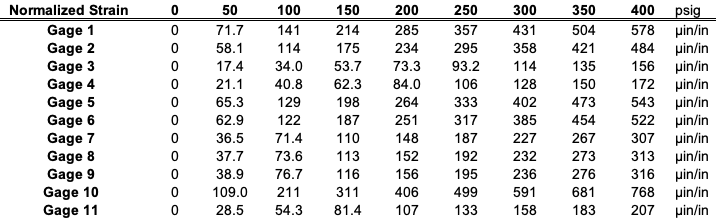
\includegraphics[width=\linewidth]{table_raw_strain}
  \centering
\end{table}
Table 1 shows the normalized strain data for each  rosette, at each pressure value. These
values comes from the method of subtracting the nominal value form the zeroed value, 
$ \epsilon_n = \epsilon_{measured} - \epsilon_0 $. The 
values were measured in microstrain, $\frac{\mu in}{in} $. Recall that the rosette configurations
held the following gages: Rosette A (1,2,3), Rosette B(4,5,6), Rosette C(7,8,9) and Rosette D(10,11).

\begin{table}[H]
  \caption{\textbf{Calculated Hoop and Axial Stresses}}
  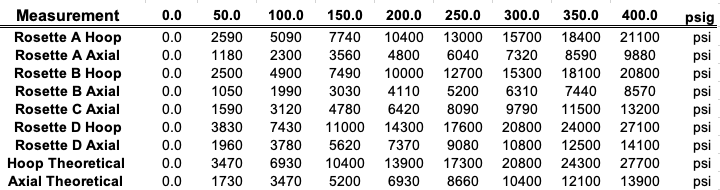
\includegraphics[width=\linewidth]{table_final_stress}
  \centering
\end{table}
Table 2 shows the calculated hoop and axial stresses for each rosette. The bottom two rows
are the theoretical values calculated from equations (12) and (13) at each pressure
level. 

% Rosette Validation 
\begin{figure} [H]
	\centering
	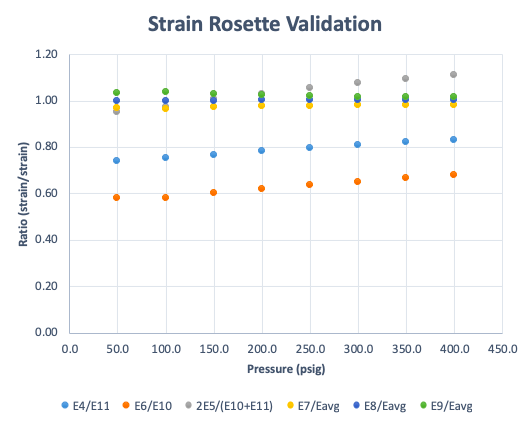
\includegraphics [width=.8\textwidth]{plot_rosette_validation}
	\caption{ \textbf{Rosette Validation Checks}}
\end{figure} 
Figure 5 displays the results from equations (1-4). These values determine how different gages within the rosettes are detecting strains which, based on configuration, should be equal.
From \textbf{Table 3}, the most accurate data is colored green, and the inaccurate data colored red. 

\begin{table}[H]
  \caption{\textbf{Strain Rosette Validation Data }}
  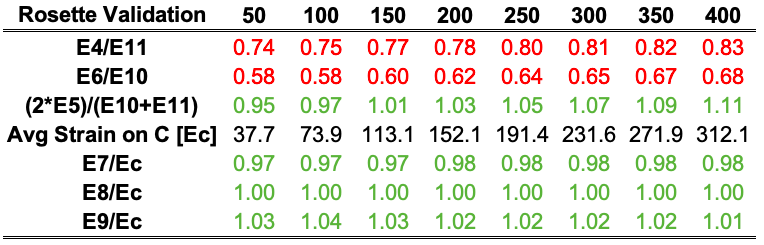
\includegraphics[width=\linewidth]{table_rosette_ratios}
  \centering
\end{table}

% Calculated axial stress 
\begin{figure} [H]
	\centering
	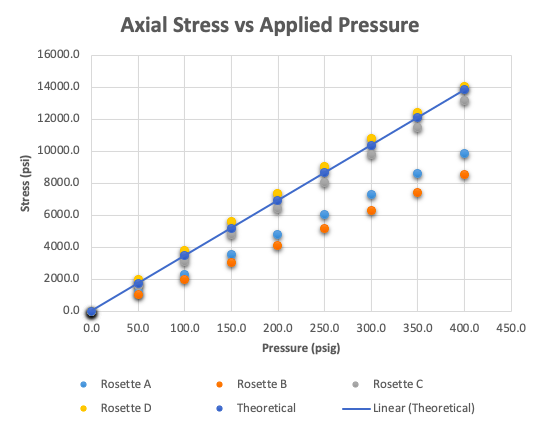
\includegraphics [width=\textwidth]{plot_axialvspressure}
	\caption{ \textbf{Calculated Axial stress vs  Pressure}}
\end{figure} 
Figure 6 shows the calculated axial stress per pressure. The blue line demonstrates the 
theoretical values. Thus, data closer to the trend line represents more accurate data relative to the theoretical values. Rosettes C and D displayed the closest resemblance, Rosettes A and B,
while linear, were not accurate. This is supported by the fact that from Figure 5 and 
Table 3, the gages on Rosettes A and B tended to be the least accurate. 

% Calculated hoop stress 
\begin{figure} [H]
	\centering
	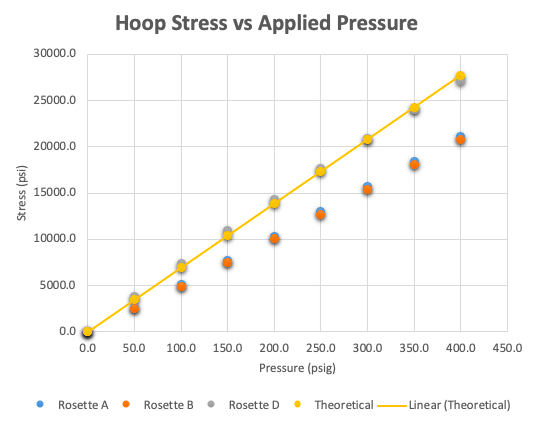
\includegraphics [width=\textwidth]{plot_hoop_measured}
	\caption{ \textbf{Calculated Hoop Stress vs Pressure}}
\end{figure} 
Figure 7 displays the calculated hoop stress for each rosette, with the theoretical values 
displayed on the yellow trend line. Thus, data closer to the line represents more accurate data, relative to the theoretical values. Recall that Rosette C, based on the position, has no hoop stress.
Once again, similar to the axial stress calculations, Rosettes A and B displayed linear but inaccurate data. The values collected from Rosette D almost mirrored the theoretical data. 

% Calc hoop vs axial 
\begin{figure} [H]
	\centering
	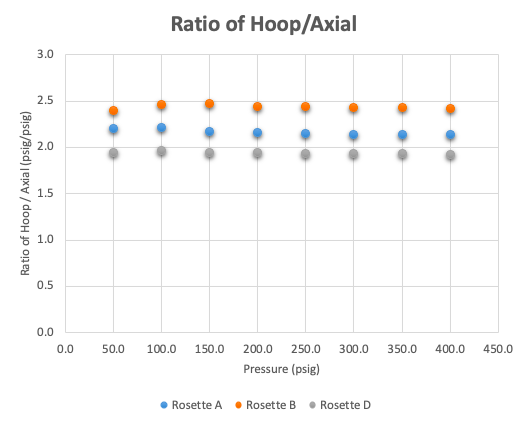
\includegraphics [width=1.0\textwidth]{plot_hoop_vs_axial}
	\caption{ \textbf{Measured Hoop vs Measured Axial}}
\end{figure} 
Based on equations (12) and (13), $ \sigma_{Hoop} $ should be twice the value of $\sigma_{Axial}$. 
Thus, the ratio of the measured hoop stress vs measured axial stress should be 2.0. Rosette D displayed the closest resemblance to 2.0, while rosettes A and B showed values higher than 2.0.
Rosette B consistently averaged a value of around 2.45, making it the least accurate value
in this measurement series. 

\begin{table}[H]
  \caption{\textbf{Table of Hoop vs Axial stress per rosette}}
  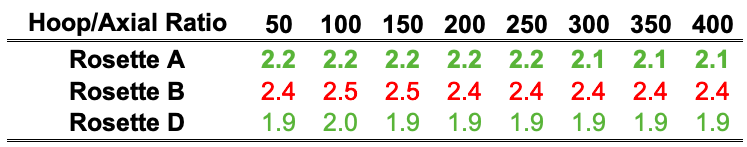
\includegraphics[width=\linewidth]{table_hoop_axial}
  \centering
\end{table}

% Axial vs theoretical 
\begin{figure} [H]
	\centering
	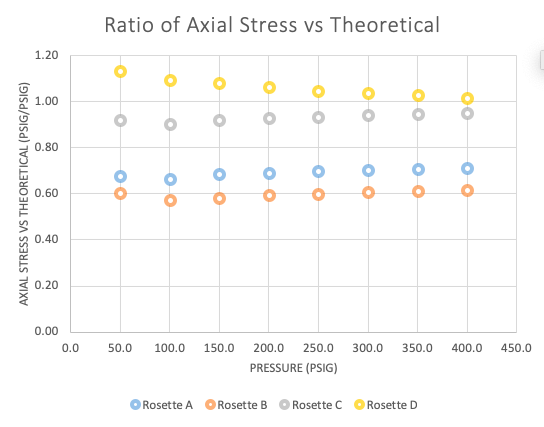
\includegraphics [width=1.0\textwidth]{plot_axialvstheor}
	\caption{ \textbf{Ratio of Measured Axial vs Theoretical Stress}}
\end{figure} 
In Figure 9, measured axial stress is analyzed. The acquired axial stress from the data reduction procedure is compared to the theoretical axial stress.

\begin{table}[H]
  \caption{\textbf{Axial stress ratio of measured vs theoretical}}
  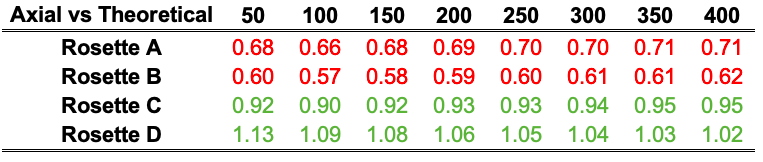
\includegraphics[width=\linewidth]{table_axial_theory}
  \centering
\end{table}
Table 5 shows the data from Figure 9. Red text signifies less accurate data, while green text signifies accurate data. 

% Calc hoop vs theoretical 
\begin{figure} [H]
	\centering
	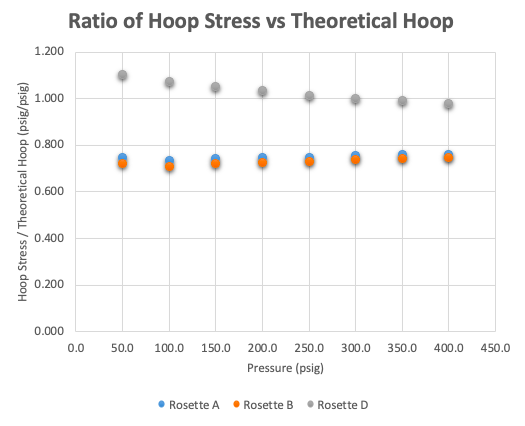
\includegraphics [width=1.0\textwidth]{plot_hoop_vs_theoretical_ratio}
	\caption{ \textbf{Hoop Stress Ratio: Measured vs Theoretical }}
\end{figure} 
Figure 10 shows the ratio of calculated hoop stress vs theoretical hoop stress. This table shows that Rosettes A and B were consistently and linearly well below the theoretical values, meaning that these rosettes were measuring a lower value than expected. Rosette D started out giving a value of 1.1, but ended up approaching the value of 1.0 as pressures increased. 

\begin{table}[H]
  \caption{\textbf{Rosettes A, B, and D: Hoop vs Theoretical Stress }}
  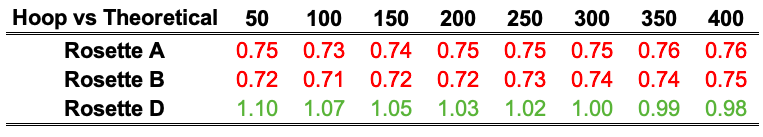
\includegraphics[width=\linewidth]{table_hoop_theoretical}
  \centering
\end{table}
\newpage

% General data 
\begin{table}[H]
  \caption{\textbf{Average R* ratios of all pressures per measurement.}}
  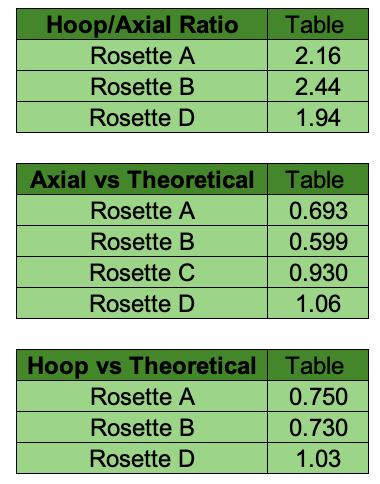
\includegraphics[width=.65\linewidth]{table_average_diff}
  \centering
\end{table}

Table 7 explains the average between every psig increment per ratio classification. This table gives a more compact summary of the other tables and figures. Here, the average differences and similarities between rosettes are more clearly and concisely conveyed. For the $\frac{\sigma_{Hoop}}{\sigma_{Axial}}$ ratio, the closer the values approach 2, the more accurate the data within the rosette. The same applies to the ratio $\frac{\sigma_{Axial Measured}}{\sigma_{Axial Theoretical}} $ . The closer to 1 these two ratios approach, the more accurate. Lower than 1 signifies a smaller than expected measured value, and a higher than 1 value shows the measured stress was larger than expected. These values came exactly from the tables above, but are simple averages of all the numbers. 
\newpage

\paragraph{Discussion}
Based on the results, Rosettes A and B were not accurate, and Rosettes C and D gave the most accurate data for both hoop and axial stresses. Not only were rosettes C and D close to the theoretical values, but all of the strain gages in these rosettes had values close to 1 in the validation equations and had an average of 2.164 and 1.942 hoop/axial ratio, respectively. Rosettes A and B had the least accuracy. This mainly comes from two factors: location and mechanical imperfections. From \textbf{Figure 2}, rosette B was placed at a location away from the center, where as rosettes A, C, and D were placed at discrete locations. The thin wall approximation assumes that all internal stresses are uniformly distributed, and this placement likely explains these differences between calculated and theoretical. Rosette B tended to give consistent data, however. All of its trends were linear as expected, and tended to, despite being inaccurate, consistently reproduce the same results. This trend of precise and inaccurate data is likely due to mechanical wear on the rosettes, age, and or tolerance issues. 

Rosette A gave consistent stress values for its own hoop and axial stresses. The ratio between hoop and axial for A was 2.164, while B had a value of 2.437. This shows that not only was rosette B inaccurate in terms of theoretical values, but it was also inaccurate at producing a value of $2\sigma_{Axial} = \sigma_{Hoop} $. As pressure increased, all rosettes tended to increase in accuracy, shown in figures 8, 9, and 10. 

% Conclusions 
\section {Conclusions and Recommendations}
\paragraph {Interpretations} 
All measurements tended to be more accurate as pressure increased. Likely, at lower pressures, the internal pressure was not distributed as evenly as it would be during higher pressures. Rosettes A and B were not reliable, but C and D were. For demonstrative/laboratory purposes, rosette B is an effective way to showcase how placements of gages can affect stress measurements. However, for industrial or research problems, the configuration of rosette B would not be effective. Also, the data supports the assumption that rosette B likely had internal mechanical issues, meaning that it could due for replacement. To measure pure axial stress, rosette C had the best location, while overall rosette D had the most accurate data set for both hoop and axial stress. Placing multiple rosettes on a single pressure vessel is an efficient way to test how accurate a set of rosettes is, and could be an effective way of determining which rosettes need replacement.


\paragraph{Reliability} Just as any other piece of mechanical equipment can begin to lose accuracy over time, strain gages are no different. Rosettes A and B tended to yield the least accurate results. Age, wear and tear, and repeated usage of the rosettes could have led to deteriorated accuracy over time. When conducting an experiment for research or more "serious" matters, check the fatigue data and general life cycle of equipment before relying on the data it receives. 

\paragraph{Placement} While not only the age and wear of rosette B could have contributed to the bad accuracy, the physical placement of the strain gage on the rosette could have made a considerable difference. Rosette D was placed dead center on the vessel, while rosette C was place at the axial end. These symmetrical placements of the rosettes played a critical role in the stress accuracy. 

\newpage
\section{What I learned}
This experiment tested our ability to not only work in teams, but to use the methods and skills we have learned through years of  class and apply them to an actual experiment. With the pressure vessel experiment, we bridged the knowledge gap between theoretical engineering and hands-on experimentation. Not only were we exposed to modern engineering instrumentation, we learned highly valuable skills in collaboration, communication, and writing proper documentation for reports. \\ 

\textbf{I testify that I have read this report and edited it as I had seen fit before submission} 


% ========== References ==========
\newpage
\section {References}
[1] Beitz, W., Kuttner, K., Davies, B., and Shields, M. (1994). 
Dubbel: Handbook of Mechanical Engineering. London: Springer-Verlag) B-42. \\ 

[2] Djeddi, Reza. (2019).Pressure Vessel Slides [pdf file]. (The University of Tennessee Knoxville). Retreived: Canvas 

% ========== Appendices ==========
\newpage
\section {Appendices}
% Raw data sheets
% Equipment list 
% Test procedure
% Hand calculations
\paragraph{Raw Strain Data}
\textbf{Appendix 1}
\begin{figure}[H]
	\centering
	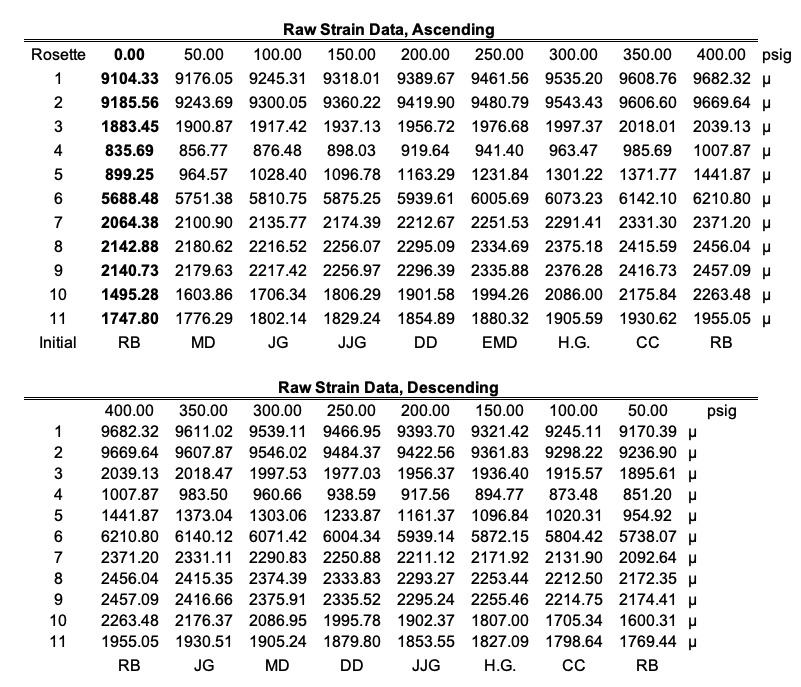
\includegraphics [width=1.0\textwidth]{appendix_rawdata}
\end{figure} 

\newpage
\paragraph{Lab Procedure}
\textbf{Appendix 2}
\begin{figure}[H]
	\centering
	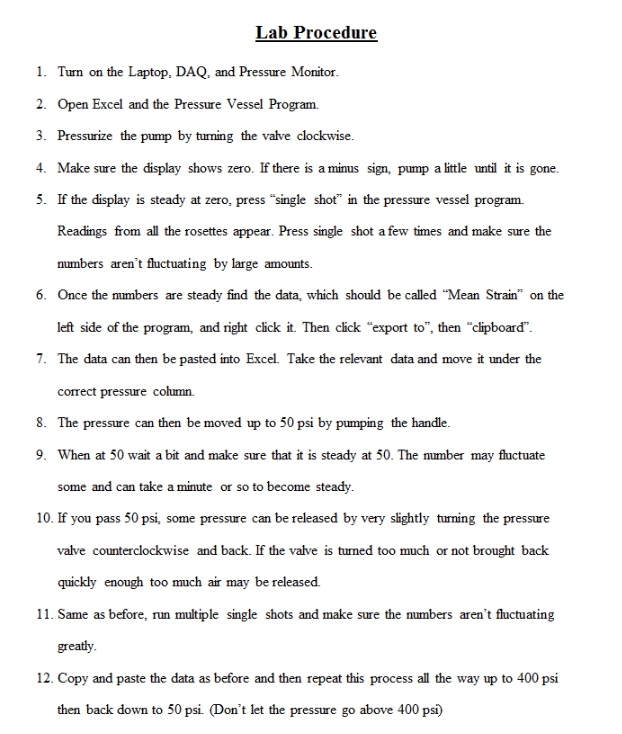
\includegraphics [width=1.0\textwidth]{appendix_procedure}
\end{figure} 

\newpage
\paragraph{Equipment Specifications}
\textbf{Appendix 3}
\begin{figure}[H]
	\centering
	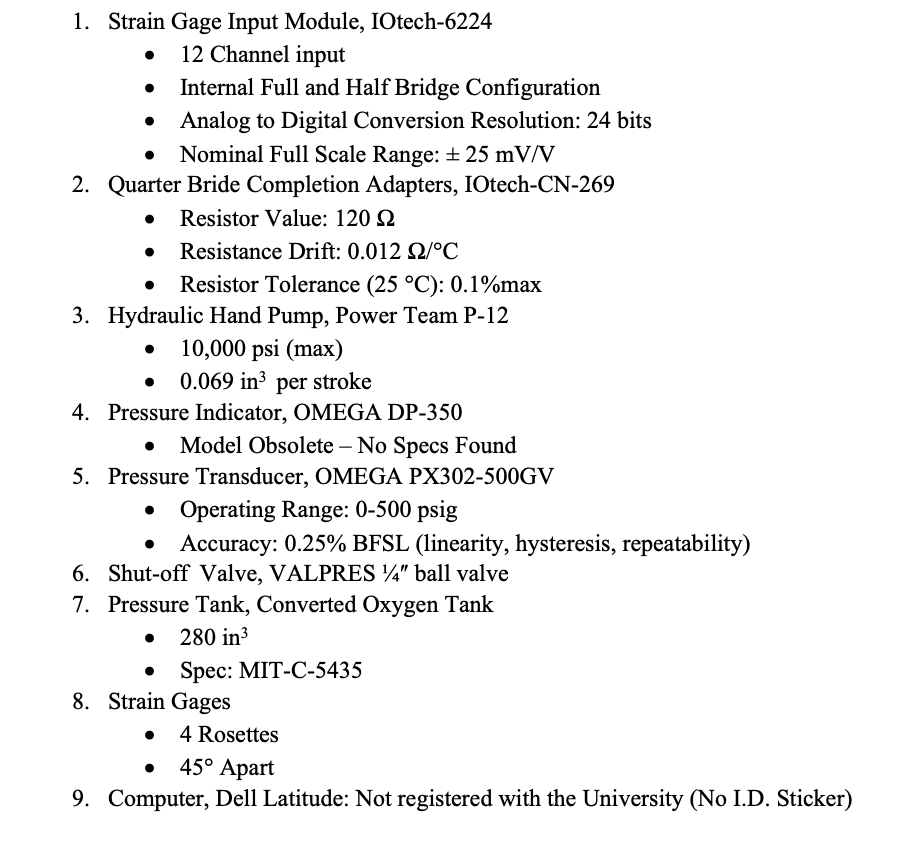
\includegraphics [width=1.0\textwidth]{appendix_equip}
\end{figure} 

% End printing here. 
\newpage
\paragraph{Hand Sample Calculations}
\end{document}
